% Author: Dr. Matthias Jung, DL9MJ
% Year: 2020
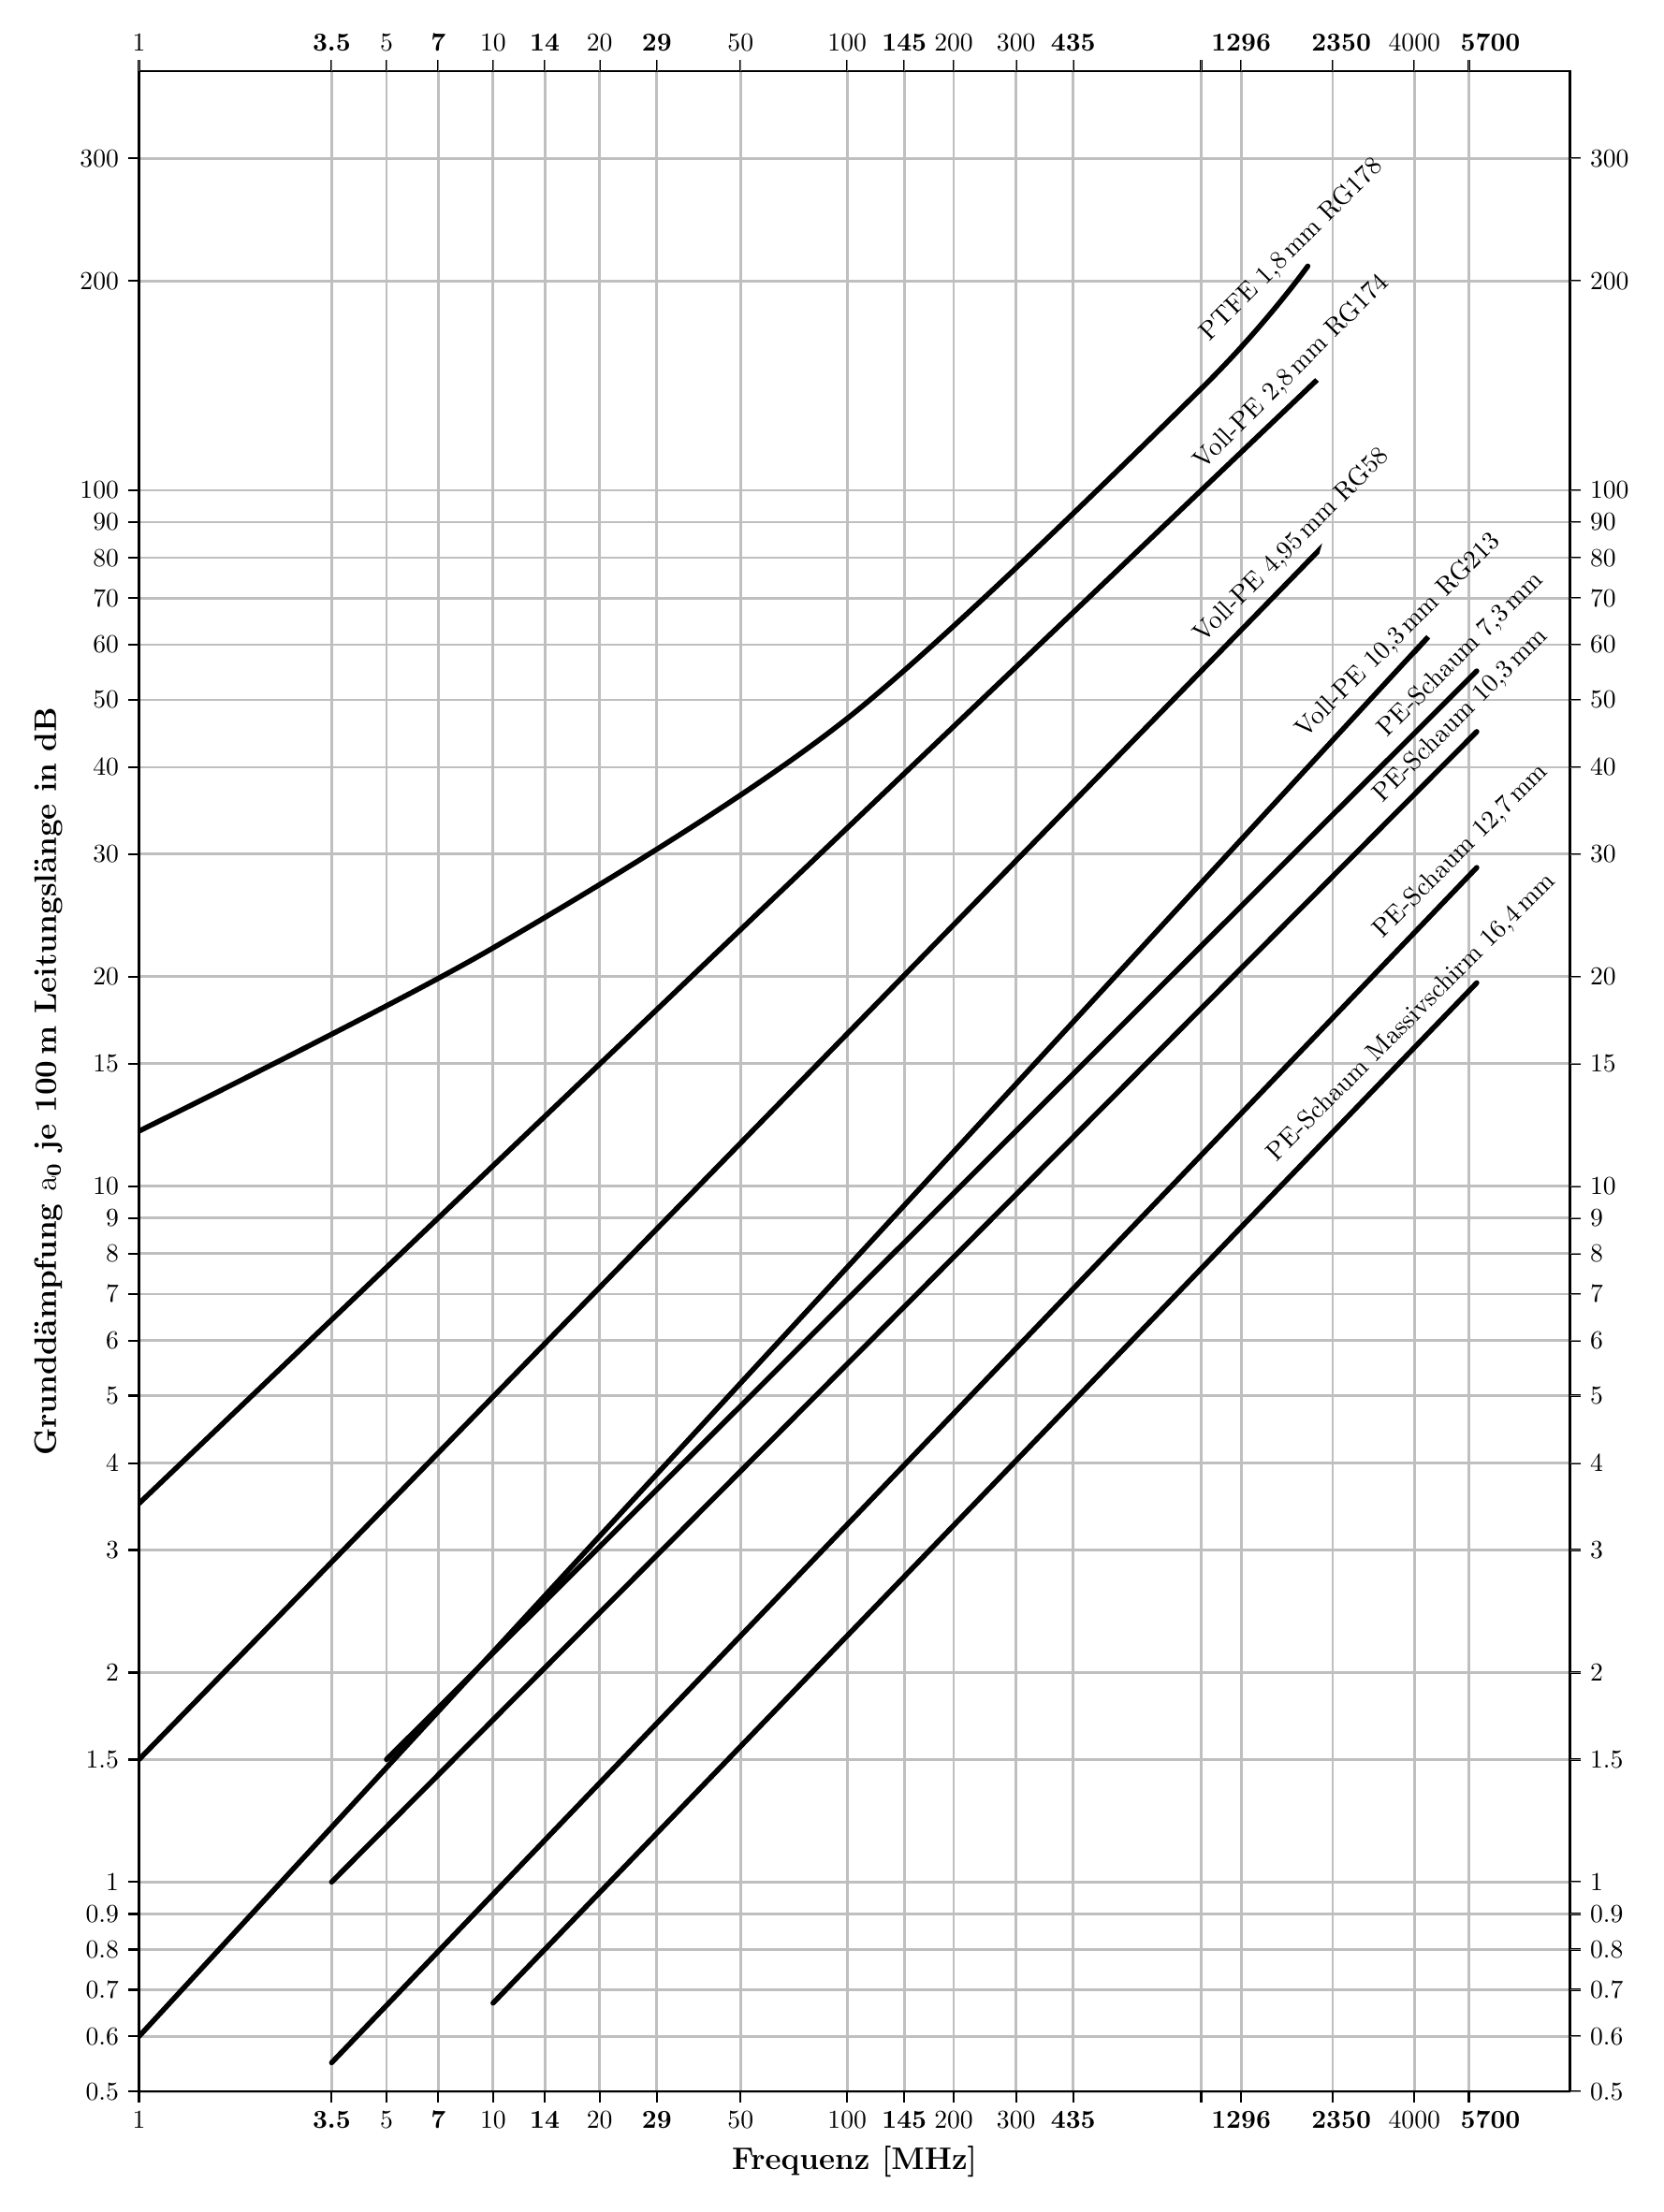
\begin{tikzpicture}
    \pgfplotsset{every axis plot}
    \pgfkeys{/pgf/number format/.cd,1000 sep={}}
    \begin{loglogaxis}
        [clip marker paths=true,legend cell align=left,
        legend style={
            at={(0.5,-0.2)},
            anchor=north},
        axis line style = thick,
        width=21cm,
        height=29cm,
        legend columns=2,
        xlabel={\textbf{\large Frequenz [MHz]}},
        ylabel={\textbf{\large Grunddämpfung $\mathbf{\mathrm{a}_0}$ je 100\,m Leitungslänge in dB}},
        xmin=1.0, xmax=11000,
        ymin=0.5, ymax=400,
        xtick={1.0,3.5,5,7,10,14,20,29,50,100,145.0,200.0,300.0,435.0,1000.0,1296.1,2350.1,4000.2,
        5700.0},
        tick align=outside,
         every tick/.style={
            black,
            thick,
        },
        xticklabels={1,\textbf{3.5},5,\textbf{7},10,\textbf{14},20,\textbf{29},50,100,\textbf{145},200,300,\textbf{435},,\textbf{1296},~~\textbf{2350},4000,~~~~~\textbf{5700}},
        ytick={0.5,0.6,0.7,0.8,0.9,1,1.5,2,3,4,5,6,7,8,9,10,15,20,30,40,50,60,70,80,90,100,200,300},
        yticklabel style={/pgf/number format/.cd,fixed,precision=1},
        yticklabel={%
          \pgfmathfloatparsenumber{\tick}%
          \pgfmathfloatexp{\pgfmathresult}%
          \pgfmathprintnumber{\pgfmathresult}%
        },
        grid=major,
        grid style={line width=1pt, draw=gray!10},
        major grid style={line width=1pt,draw=gray!50}
        ]
     
        \def\gradzahl{45}
    
        \addplot[smooth, line width=2pt, line cap=round] coordinates
        {(   1,  12.0)
         (  10,  22.0)
         ( 100,  47.0)
         (1000, 140.0)
         (2000, 210.0)
         } node[above,pos=1,rotate=\gradzahl] {PTFE 1,8\,mm RG178}; % RG 178
    
    
        \addplot[smooth, line width=2pt, line cap=round] coordinates
        {(   1,  3.5)
         (1000,  100.0)
         (2000,  140.0)
         } node[above,pos=1,rotate=\gradzahl] {Voll-PE 2,8\,mm RG174}; % RG 174
    
        \addplot[smooth, line width=2pt] coordinates
        {(   1,  1.5)
         (1000, 55.0)
         (2000, 79.0)
         } node[above,pos=1,rotate=\gradzahl] {Voll-PE 4,95\,mm RG58}; % RG 58
    
    
        \addplot[smooth, line width=2pt, line cap=round] coordinates
        {(   1,  0.6)
         (2000, 40.0)
         (4000, 58.55)
         } node[above,pos=1,rotate=\gradzahl] {Voll-PE  10,3\,mm RG213}; % RG 213
    
        \addplot[smooth, line width=2pt, line cap=round] coordinates
        {(   5, 1.5)
         (6000, 55.0)
         } node[above,pos=1,rotate=\gradzahl] {PE-Schaum 7,3\,mm};
    
    
        \addplot[smooth, line width=2pt, line cap=round] coordinates
        {( 3.5,  1.0)
         (6000, 45.0)
         } node[above,pos=1,rotate=\gradzahl] {PE-Schaum 10,3\,mm};
    
        \addplot[smooth, line width=2pt, line cap=round] coordinates
        {( 3.5,  0.55)
         (6000, 28.70)
         } node[above,pos=1,rotate=\gradzahl] {PE-Schaum 12,7\,mm};
    
    
        \addplot[smooth, line width=2pt, line cap=round] coordinates
        {( 10,  0.67)
         (6000, 19.60)
         } node[above,pos=0.95,rotate=\gradzahl] {PE-Schaum Massivschirm 16,4\,mm};
    
    \end{loglogaxis}%
    \begin{loglogaxis}[
        axis y line*=right,
        axis x line*=top,
        ymin=0.5, ymax=400,
        width=21cm,
        height=29cm,
        tick align=outside,
        xmin=1,xmax=11000,
        xticklabels=none,
        ytick={0.5,0.6,0.7,0.8,0.9,1,1.5,2,3,4,5,6,7,8,9,10,15,20,30,40,50,60,70,80,90,100,200,300},
        yticklabel style={/pgf/number format/.cd,fixed,precision=1},
        yticklabel={%
          \pgfmathfloatparsenumber{\tick}%
          \pgfmathfloatexp{\pgfmathresult}%
          \pgfmathprintnumber{\pgfmathresult}%
        },
        xminorticks=false,
        xtick={1.0,3.5,5,7,10,14,20,29,50,100,145.0,200.0,300.0,435.0,1000.0,1296.1,2350.1,4000.2,
        5700.0},
        xticklabels={1,\textbf{3.5},5,\textbf{7},10,\textbf{14},20,\textbf{29},50,100,\textbf{145},200,300,\textbf{435},,\textbf{1296},~~\textbf{2350},4000,~~~~~\textbf{5700}},
        ]
    \end{loglogaxis}%
\end{tikzpicture}